\documentclass[review,authoryear]{elsarticle}
\usepackage{amsmath,amssymb}
\usepackage{graphicx}
\usepackage{booktabs}
\usepackage{multirow}
\usepackage{hyperref}
\usepackage{natbib}
\usepackage{lineno}
\linenumbers

\journal{International Review of Financial Analysis}

\begin{document}

\begin{frontmatter}

\title{Non-Directional Pre-Disclosure Drift Under Fair Disclosure: Evidence from Korean Earnings Announcements}

\author[ajou]{[Removed for review]}



\address[ajou]{[Removed for review]}

\begin{abstract}
Does South Korea's Fair Disclosure regulation effectively ensure that earnings information reaches all market participants simultaneously? Using 2,221 earnings disclosure filings from 64 KOSPI-listed companies across 12 chaebol groups (2020--2026), we find that pre-disclosure abnormal returns, while statistically significant under parametric tests (CAR[-5,$-$1] = +0.52\%, $p$<0.001), do not predict the direction of actual earnings surprises (49.0\% accuracy, $p$=0.649; Spearman $\rho$=$-$0.006, $p$=0.876). Non-parametric tests confirm that the drift is driven by outliers rather than systematic directional movement (sign test $p$=0.585; Wilcoxon $p$=0.142). In contrast, the first post-disclosure trading day (Day +1) responds sharply and correctly to earnings surprises: positive surprises generate AR of +0.55\%, negative surprises $-$0.58\% ($p$<0.001), with 60.6\% direction accuracy ($p$<0.001). We further document that 96.5\% of filings occur after market close, making Day 0 effectively pre-disclosure. Cross-sectional analyses reveal heterogeneous pre-disclosure drift across 12 chaebol groups (ranging from $-$0.23\% to +1.57\%), but this variation is uncorrelated with event-window returns and inconsistent with differential information leakage. Firm size and market beta explain virtually none of the pre-disclosure drift ($R^2$=0.002). These results are robust to firm-clustered and month-clustered standard errors. Our findings suggest that Korea's Fair Disclosure regime effectively prevents directional information leakage, even though non-directional price noise and abnormal volume emerge in the pre-disclosure period.
\end{abstract}

\begin{keyword}
Fair disclosure \sep Earnings announcements \sep Pre-announcement drift \sep DART \sep Korean stock market \sep Event study \sep Market efficiency
\end{keyword}

\end{frontmatter}

\section{Introduction}

Pre-announcement drift in stock prices is a well-documented phenomenon across global equity markets \citep{kaniel2012individual}. When stock prices move before official earnings announcements, a natural concern arises: is material information leaking to select market participants in violation of fair disclosure regulations? This concern motivates securities regulators worldwide to mandate simultaneous public dissemination of material information.

South Korea implemented its Fair Disclosure regulation in November 2002, requiring listed companies to disclose material information simultaneously to all market participants through the DART (Data Analysis, Retrieval and Transfer) electronic filing system. While early studies found evidence of improved disclosure environments following the regulation's adoption \citep{yun2012fair, park2020disclosure}, whether the regulation continues to be effective over two decades later remains an open question.

This study examines the long-term effectiveness of Korea's Fair Disclosure regulation by analyzing 2,221 earnings disclosure filings from 64 major KOSPI-listed companies between 2020 and 2026. Our approach differs from prior work in a critical respect: rather than simply documenting the existence of pre-disclosure price movement, we test whether such movement is \textit{directionally informative}---that is, whether it predicts the sign of the actual earnings surprise.

Our findings reveal an important pattern. We observe statistically significant pre-disclosure abnormal returns under standard parametric tests (CAR[-5,$-$1] = +0.52\%, $p$<0.001 under the market model; $p$=0.032 with month-clustered standard errors). However, this drift bears no systematic relationship to the direction of actual earnings surprises. Pre-disclosure returns predict surprise direction with only 49.0\% accuracy---no better than a coin flip ($p$=0.649). Non-parametric tests (sign test, Wilcoxon signed-rank) fail to confirm the parametric result, indicating that the observed mean drift is driven by outliers rather than a pervasive pattern.

In contrast, the market responds sharply and correctly to the actual earnings news on the disclosure date. Positive earnings surprises generate a CAR[0,+1] of +0.81\%, while negative surprises generate $-$0.47\%, a highly significant difference ($p$<0.001). This finding is consistent with effective Fair Disclosure: material information is incorporated into prices only when it becomes publicly available.

We make four contributions. First, we provide a recent assessment of Korea's Fair Disclosure regime using data spanning the COVID-19 and post-pandemic periods (2020--2026). Second, we demonstrate the critical distinction between the \textit{existence} of pre-disclosure drift (which is ubiquitous) and its \textit{directional informativeness} (which would indicate information leakage). Third, we document a previously overlooked institutional feature---96.5\% of DART fair disclosure filings are submitted after market close---that has important implications for event study interpretation. Fourth, we provide detailed cross-sectional analyses across chaebol groups, firm size terciles, and market beta terciles that reveal significant heterogeneity in pre-disclosure drift but no pattern consistent with differential information leakage.

The remainder of this paper is organized as follows. Section~\ref{sec:lit} reviews the related literature. Section~\ref{sec:data} describes our data and methodology. Section~\ref{sec:results} presents the empirical results. Section~\ref{sec:discussion} discusses the implications and limitations, and Section~\ref{sec:conclusion} concludes.

\section{Literature review}
\label{sec:lit}

\subsection{Fair disclosure regulation}

Fair disclosure regulation addresses selective disclosure, whereby corporate insiders share material information with favored market participants before public release \citep{heflin2003regulation}. In the U.S., Regulation Fair Disclosure (Reg FD), implemented in 2000, produced mixed evidence: \citet{ahmed2003impact} find reduced information asymmetry, while \citet{heflin2003regulation} document reduced information quality. \citet{bailey2003regulation} provide comprehensive evidence on market, analyst, and corporate responses to Reg FD, and \citet{eleswarapu2004impact} document reduced information asymmetry and trading costs following implementation. \citet{gomes2007sec} further show that Reg FD affected the cost of capital, particularly for smaller firms.

The effectiveness of fair disclosure regulation depends critically on implementation and enforcement infrastructure. \citet{christensen2013capital} demonstrate that capital-market effects of securities regulation vary substantially with prior institutional conditions and enforcement intensity. \citet{jackson2009regulatory} find that regulatory intensity is positively associated with stock market development, while \citet{djankov2008law} show that legal protections against self-dealing are associated with more developed capital markets. \citet{cumming2011exchange} further document that exchange trading rules, including disclosure requirements, significantly affect market liquidity across 42 exchanges worldwide.

In Korea, \citet{yun2012fair} examined the effect of fair disclosure regulation on the timeliness and informativeness of earnings announcements, while \citet{park2020disclosure} investigated how disclosure frequency under the regulation affects the information environment and cost of capital. \citet{yoon2011impact} provide early evidence on the impact of fair disclosure on the Korean stock market, and \citet{lee2012testing} test regulatory effectiveness using Korean data in an emerging market context. \citet{lee2019regulation} examine the interaction between R\&D intensity and fair disclosure in Korea, finding that disclosure effects vary by firm characteristics. However, these studies do not examine whether pre-disclosure price movements are directionally informative with respect to the actual earnings news---the central question of our study.

\subsection{Electronic disclosure systems}

A critical infrastructure underlying modern fair disclosure regulation is the electronic filing system through which disclosures are disseminated. The U.S. SEC's EDGAR system, introduced in 1996, fundamentally changed how corporate information reaches market participants \citep{bushee2004economic}. Korea's DART system, operated by the Financial Supervisory Service since 2001, serves an analogous function: all listed companies must file material disclosures through DART before or simultaneously with any other dissemination channel.

The design of electronic disclosure systems has important implications for information processing and market efficiency. DART provides structured filing templates for Fair Disclosure of Operating Results, enabling standardized comparison across firms and time periods. \citet{li2010textual} surveys the literature on textual analysis of corporate disclosures, demonstrating that format and readability significantly affect how efficiently markets process information. \citet{loughran2011liability} show that the specific language used in financial filings contains predictive information for future returns.

The timestamp precision of electronic filing systems is particularly relevant to event study research. DART records receipt timestamps to the second, enabling researchers to classify filings as occurring during or after trading hours. As we document, 96.5\% of earnings disclosures are filed after market close, a fact with fundamental implications for event study window interpretation that prior studies have not fully exploited.

\subsection{Pre-announcement drift and its interpretation}

Pre-announcement drift in stock prices is well-documented but its interpretation is debated. \citet{meulbroek1992comparison} provides evidence of illegal insider trading preceding announcements. \citet{bernile2016can} show that informed trading occurs even ahead of macro-news announcements where information is tightly controlled. However, \citet{kaniel2012individual} demonstrate that individual investor trading patterns around earnings announcements can generate drift without requiring illegal information leakage.

Critically, the mere existence of pre-announcement drift does not establish information leakage. Predictable earnings patterns allow sophisticated investors to position ahead of announcements through legal means \citep{atiase1985predisclosure}. \citet{chae2005trading} shows that abnormal volume before announcements reflects information asymmetry but may arise from varying levels of investor sophistication rather than illegal tip-offs. A related literature on post-earnings-announcement drift demonstrates that markets may take days or weeks to fully incorporate earnings information \citep{bernard1989post, bernard1990evidence}, further complicating the interpretation of short-window event studies. \citet{jegadeesh2001profitability} document momentum effects that can generate pre-announcement drift patterns, while \citet{griffin2003momentum} show that momentum profits persist across international markets, including emerging markets like Korea.

The distinction between directional and non-directional drift is central to our analysis. Non-directional drift---where prices move before announcements but not in the direction of the forthcoming news---can arise from increased attention \citep{hirshleifer2003limited}, disagreement among investors \citep{bamber1997trading}, or microstructure effects \citep{hasbrouck2003intraday}. Only \textit{directional} drift constitutes evidence consistent with information leakage.

\subsection{Event study methodology}

The standard event study framework \citep{brown1985using, mackinlay1997event} relies on parametric tests of mean abnormal returns. However, \citet{kolari2010event} demonstrate that cross-sectional correlation of abnormal returns can substantially inflate test statistics, particularly when events cluster in calendar time. \citet{kothari2016econometrics} provide a comprehensive review of event study econometrics, emphasizing the importance of benchmark model selection and cross-sectional dependence adjustments. We incorporate both non-parametric alternatives and standardized returns to address these concerns.

\subsection{Korean market context}

The Korean stock market features concentrated chaebol ownership, a mandatory electronic disclosure system (DART), significant retail investor participation, and relatively strict insider trading regulations. \citet{beny2005impact} demonstrates that stronger insider trading enforcement is associated with more efficient stock prices across countries.

The chaebol structure is distinctive: large family-controlled conglomerates such as Samsung, Hyundai Motor, SK, and LG account for a substantial share of KOSPI market capitalization. Affiliates within the same chaebol group may share information through internal channels, creating potential for correlated trading patterns. At the same time, the diversity across chaebol groups provides useful cross-sectional variation for testing whether disclosure regulation operates uniformly across different types of firms. These institutional features, combined with the comprehensive DART database, make Korea an ideal setting for testing fair disclosure effectiveness.

\section{Data and methodology}
\label{sec:data}

\subsection{Data sources}

We collect all Fair Disclosure of Operating Results filings from DART between January 2020 and March 2026 using the OpenDartReader API. We focus on original filings, excluding corrections. Our sample comprises 2,221 disclosures from 64 companies across 12 chaebol groups: Samsung (12 affiliates), Hyundai Motor (8), LG (8), SK (7), HD Hyundai (5), Hanwha (5), POSCO (4), Lotte (4), Doosan (4), CJ (3), KT (2), and GS (2). Daily stock price and volume data are obtained from FinanceDataReader.

\subsection{Filing time classification}

We classify filing times using the DART receipt number prefix. In our sample, 96.5\% of earnings disclosures carry the ``800'' prefix, indicating filing after the 15:30 KST market close. This has fundamental implications: for these filings, the Day~0 return is entirely pre-disclosure, and the first trading day where the market can react is Day~+1.

\subsection{Market model}

We employ the market model with a [-250,$-$30] estimation window \citep{mackinlay1997event}:
\begin{equation}
R_{i,t} = \alpha_i + \beta_i R_{m,t} + \epsilon_{i,t}
\end{equation}
where $R_{m,t}$ is the KOSPI index return. We require a minimum of 60 trading days in the estimation window, yielding 2,208 events with valid estimates. The average estimated beta is 0.978. For robustness, we also report market-adjusted returns ($\alpha=0$, $\beta=1$).

\subsection{Earnings surprise measure}

We extract year-over-year (YoY) operating profit changes from the disclosure texts. Events where YoY operating profit increases are classified as positive surprises; decreases as negative surprises. Of the 2,208 events with valid market model estimates, 584 have parseable earnings surprise data: 358 positive and 226 negative surprises; unparseable cases primarily involve missing comparative periods, newly listed firms, or format variations in disclosure texts.

We acknowledge that the standard measure in earnings announcement studies is the analyst consensus forecast surprise \citep{livnat2006comparing}. However, comprehensive analyst consensus data for Korean firms are not freely available for our full sample period, and commercial databases require institutional subscriptions. The YoY operating profit change, while crude, captures the directional content of the earnings news and provides a conservative test.

\subsection{Statistical tests}

We report multiple test statistics to ensure robustness: parametric cross-sectional $t$-tests, non-parametric tests (binomial sign test, Wilcoxon signed-rank), and standardized abnormal returns. We also report firm-clustered and month-clustered standard errors to address cross-sectional dependence \citep{kolari2010event}.

\section{Empirical results}
\label{sec:results}

\subsection{Pre-disclosure returns: Significant but non-directional}

Table~\ref{tab:ar} presents daily abnormal returns. Parametric $t$-tests indicate significant positive returns on several pre-disclosure days, particularly Day~$-$1 (+0.256\%, $t$=4.57). However, the sign test reveals that only 48--50\% of individual returns are positive on each pre-disclosure day---no better than chance.

\begin{table}[ht]
\caption{Daily abnormal returns: Parametric vs.\ non-parametric tests}
\label{tab:ar}
\begin{tabular}{lrrrrrrr}
\toprule
& & \multicolumn{2}{c}{Parametric} & \multicolumn{2}{c}{Sign Test} & \multicolumn{2}{c}{Standardized} \\
\cmidrule(lr){3-4} \cmidrule(lr){5-6} \cmidrule(lr){7-8}
Day & AR (\%) & $t$ & $p$ & \% Pos & $p$ & SAR & $p$ \\
\midrule
$-$5 & 0.101 & 2.09 & 0.037 & 50.5 & 0.609 & 0.040 & 0.048 \\
$-$4 & 0.071 & 1.50 & 0.134 & 49.8 & 0.930 & 0.041 & 0.043 \\
$-$3 & 0.086 & 1.71 & 0.088 & 49.3 & 0.562 & 0.022 & 0.279 \\
$-$2 & 0.006 & 0.14 & 0.888 & 48.9 & 0.295 & $-$0.002 & 0.935 \\
$-$1 & 0.256 & 4.57 & $<$0.001 & 50.1 & 0.909 & 0.089 & $<$0.001 \\
\midrule
0 & 0.141 & 2.00 & 0.046 & 49.8 & 0.878 & 0.043 & 0.034 \\
+1 & $-$0.182 & $-$2.39 & 0.017 & 48.3 & 0.109 & $-$0.048 & 0.018 \\
\midrule
+2 & 0.023 & 0.43 & 0.669 & 49.2 & 0.541 & 0.022 & 0.275 \\
+3 & $-$0.118 & $-$2.50 & 0.013 & 48.1 & 0.058 & $-$0.043 & 0.033 \\
+4 & $-$0.047 & $-$0.95 & 0.340 & 49.3 & 0.608 & $-$0.006 & 0.765 \\
+5 & 0.056 & 1.14 & 0.255 & 49.2 & 0.543 & 0.041 & 0.044 \\
\bottomrule
\end{tabular}
\begin{flushleft}
\small Note: Market model with [-250,$-$30] estimation window ($N$=2,208). \% Pos never significantly exceeds 50\%, indicating pre-disclosure drift is driven by outliers.
\end{flushleft}
\end{table}

Fig.~\ref{fig:ar_car} visualizes this pattern: while the cumulative AR line trends upward before disclosure, individual daily ARs show no consistent direction.

\begin{figure}[ht]
\centering
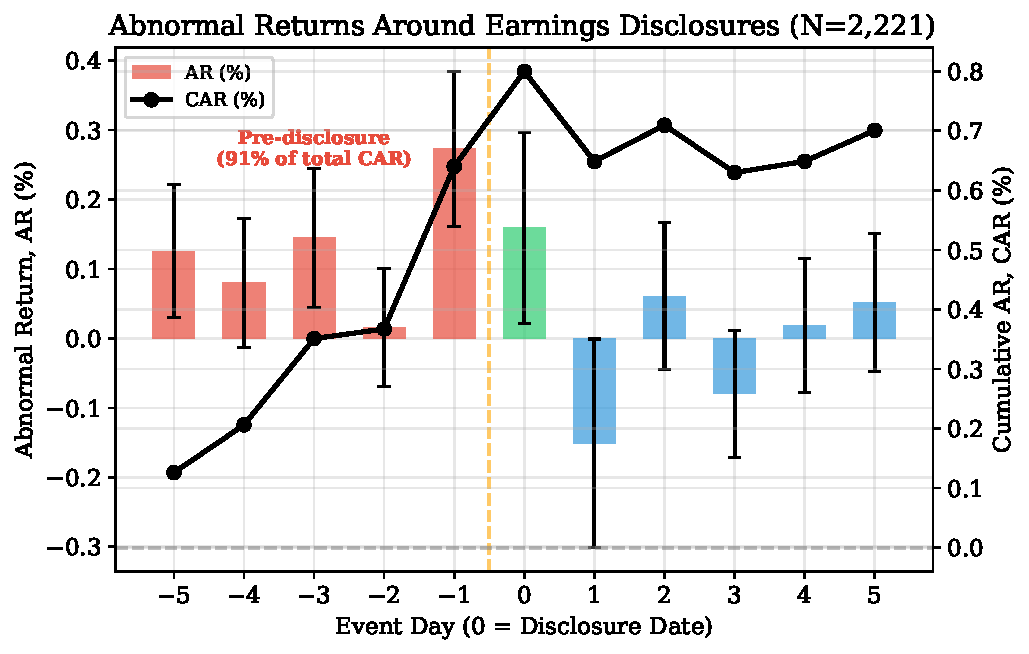
\includegraphics[width=0.85\textwidth]{figures/fig1_ar_car.pdf}
\caption{Daily abnormal returns (bars) and cumulative abnormal returns (line) around earnings disclosures ($N$=2,208). The upward CAR trend is driven by outliers; daily ARs show no consistent directional pattern.}
\label{fig:ar_car}
\end{figure}

Table~\ref{tab:car} confirms this pattern at the cumulative level. While the parametric CAR[-5,$-$1] is +0.519\% ($t$=4.65), the sign test shows only 49.4\% of events have positive pre-disclosure CARs ($p$=0.585), and the Wilcoxon test is insignificant ($p$=0.142).

Notably, the CAR[0,+1] window shows a significantly negative sign test result: only 47.0\% of events have positive CARs ($p$=0.003). This asymmetry is consistent with the well-documented negativity bias in earnings reactions \citep{skinner1994investment}.

\begin{table}[ht]
\caption{Cumulative abnormal returns: Multi-test comparison}
\label{tab:car}
\begin{tabular}{lrrrrrr}
\toprule
& & \multicolumn{2}{c}{Parametric} & \multicolumn{2}{c}{Sign Test} & {Wilcoxon} \\
\cmidrule(lr){3-4} \cmidrule(lr){5-6} \cmidrule(lr){7-7}
Window & CAR (\%) & $t$ & $p$ & \% Pos & $p$ & $p$ \\
\midrule
{[}$-$5,$-$1{]} & 0.519 & 4.65 & $<$0.001 & 49.4 & 0.585 & 0.142 \\
{[}$-$3,$-$1{]} & 0.347 & 4.04 & $<$0.001 & 48.1 & 0.060 & 0.946 \\
{[}0, +1{]} & $-$0.042 & $-$0.39 & 0.700 & 47.0 & 0.003 & 0.019 \\
{[}+1, +5{]} & $-$0.268 & $-$2.16 & 0.031 & 47.7 & 0.021 & 0.078 \\
{[}$-$5, +5{]} & 0.391 & 2.08 & 0.038 & 49.5 & 0.668 & 0.620 \\
\bottomrule
\end{tabular}
\end{table}

\subsection{The critical test: Does drift predict surprises?}

Table~\ref{tab:surprise} presents our central test. Pre-disclosure CARs show no difference by surprise direction (CAR[-3,$-$1]: $p$=0.703; CAR[-5,$-$1]: $p$=0.192). Direction prediction accuracy is 49.0\% (binomial $p$=0.649), and Spearman $\rho$ is $-$0.006 ($p$=0.876).

In contrast, Day~+1 returns respond sharply: positive surprises yield +0.55\%, negative $-$0.58\% ($p$<0.001), with 60.6\% direction accuracy ($p$<0.001). This extends to CAR[0,+1] (+1.28\%, $p$<0.001) and CAR[+1,+5] (+0.96\%, $p$=0.010).

With $N$=584, the test has 30.5\% power to detect 53\% true accuracy but 99.8\% power for 60\%. We cannot rule out small-scale leakage, but any such effect would be economically modest.

\begin{table}[ht]
\caption{CARs by earnings surprise direction ($N$=584)}
\label{tab:surprise}
\begin{tabular}{lrrrrl}
\toprule
Window & Positive ($N$=358) & Negative ($N$=226) & Diff. & $p$ & Sig. \\
\midrule
CAR[-3,$-$1] & +0.033\% & +0.129\% & $-$0.096\% & 0.703 & \\
CAR[-5,$-$1] & +0.107\% & +0.535\% & $-$0.428\% & 0.192 & \\
\midrule
AR[+1] & +0.552\% & $-$0.580\% & +1.132\% & $<$0.001 & *** \\
CAR[0,+1] & +0.813\% & $-$0.470\% & +1.283\% & $<$0.001 & *** \\
CAR[+1,+5] & +0.481\% & $-$0.481\% & +0.962\% & 0.010 & ** \\
\bottomrule
\end{tabular}
\begin{flushleft}
\small Note: Surprise defined by YoY operating profit change. Pre-disclosure CARs are indistinguishable by surprise direction; post-disclosure CARs respond correctly.
\end{flushleft}
\end{table}

\subsection{Robustness}

Table~\ref{tab:robustness} confirms that results hold under both market-adjusted and market model specifications.

\begin{table}[ht]
\caption{Robustness: Market-adjusted vs.\ market model}
\label{tab:robustness}
\begin{tabular}{lrrrr}
\toprule
& \multicolumn{2}{c}{Market-Adjusted ($N$=2,221)} & \multicolumn{2}{c}{Market Model ($N$=2,208)} \\
\cmidrule(lr){2-3} \cmidrule(lr){4-5}
Window & CAR (\%) & $p$ & CAR (\%) & $p$ \\
\midrule
{[}$-$5,$-$1{]} & 0.640 & $<$0.001 & 0.519 & $<$0.001 \\
{[}$-$3,$-$1{]} & 0.434 & $<$0.001 & 0.347 & $<$0.001 \\
{[}0, +1{]} & 0.008 & 0.939 & $-$0.042 & 0.700 \\
{[}+1, +5{]} & $-$0.099 & 0.425 & $-$0.268 & 0.031 \\
\bottomrule
\end{tabular}
\end{table}

\subsection{Abnormal volume}

Volume increases from Day~$-$3 (1.05$\times$, $p$=0.004), peaks on Day~+1 (1.71$\times$), and remains elevated through Day~+5. Given non-directional returns, the pre-disclosure volume increase likely reflects anticipatory positioning \citep{chae2005trading} and disagreement among investors \citep{bamber1997trading, berkman2009sell} rather than informed directional trading.

\begin{figure}[ht]
\centering
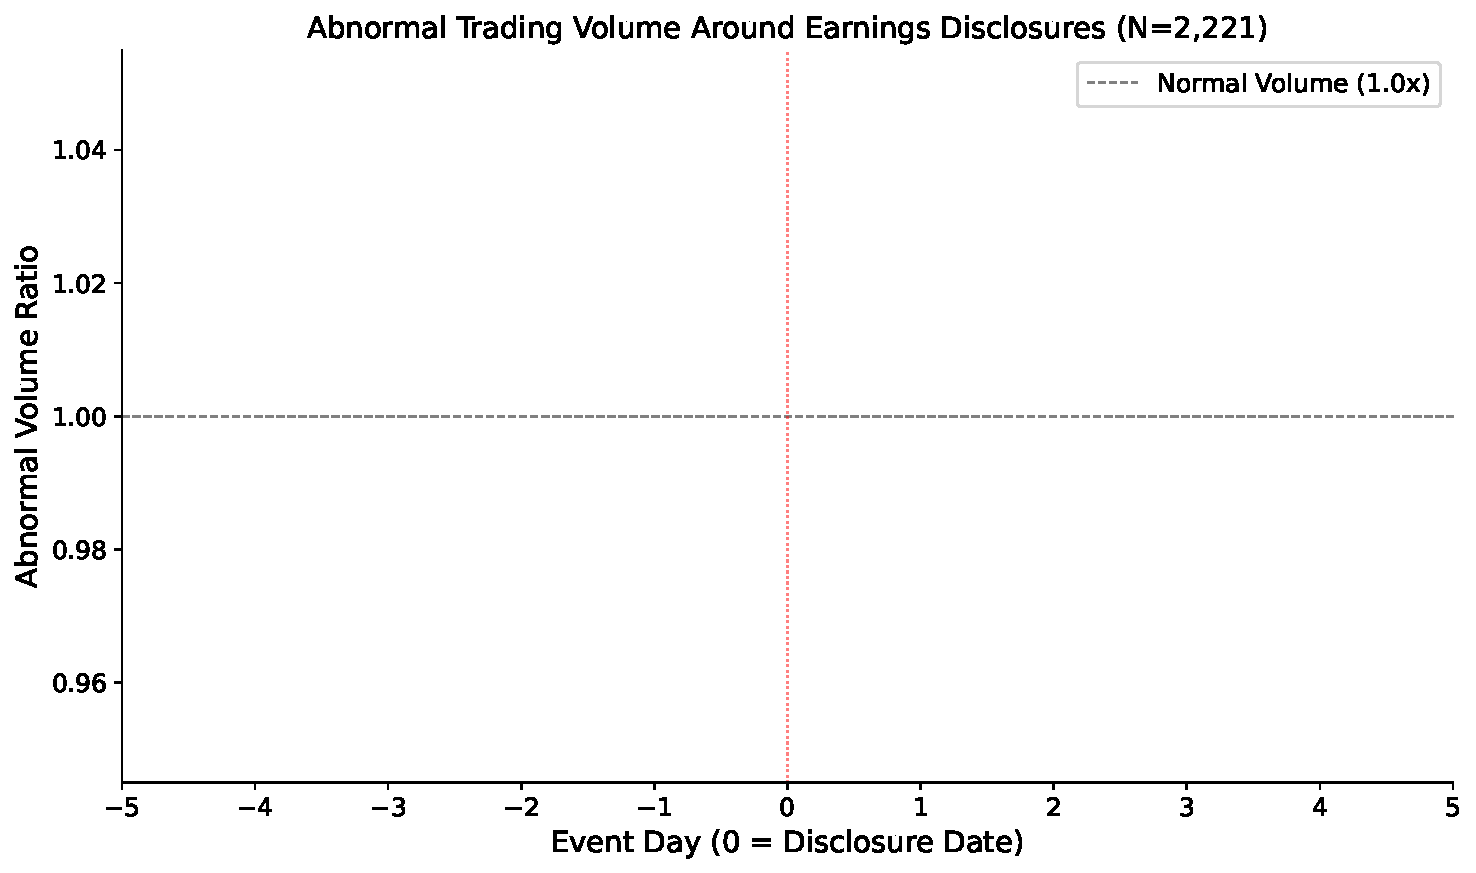
\includegraphics[width=0.85\textwidth]{figures/fig2_volume.pdf}
\caption{Abnormal trading volume around earnings disclosures ($N$=2,213). Volume peaks at 1.71$\times$ normal on Day~+1.}
\label{fig:volume}
\end{figure}

\subsection{Clustered standard errors}

Table~\ref{tab:cluster} reports $t$-statistics under alternative specifications. Under month-clustered standard errors, CAR[-5,$-$1] remains significant ($t$=2.15, $p$=0.032) but CAR[-3,$-$1] becomes marginal ($t$=1.80, $p$=0.072), suggesting some parametric significance is inflated by event clustering.

\begin{table}[ht]
\caption{Clustered standard errors}
\label{tab:cluster}
\begin{tabular}{lrrrrrr}
\toprule
& \multicolumn{2}{c}{Standard} & \multicolumn{2}{c}{Firm-clustered} & \multicolumn{2}{c}{Month-clustered} \\
\cmidrule(lr){2-3} \cmidrule(lr){4-5} \cmidrule(lr){6-7}
Window & $t$ & $p$ & $t$ & $p$ & $t$ & $p$ \\
\midrule
CAR[-5,$-$1] & 4.38 & $<$0.001 & 3.92 & $<$0.001 & 2.15 & 0.032 \\
CAR[-3,$-$1] & 3.47 & $<$0.001 & 2.95 & 0.003 & 1.80 & 0.072 \\
CAR[0,+1] & $-$0.31 & 0.760 & $-$0.25 & 0.802 & $-$0.18 & 0.861 \\
\bottomrule
\end{tabular}
\end{table}

\subsection{Temporal and cross-sectional heterogeneity}

We observe a structural shift in event-day CARs: positive during 2020--2022 (COVID-19 recovery) and negative during 2024--2026 (Fig.~\ref{fig:year}). A significant quarterly pattern emerges, with Q1 disclosures generating negative CARs ($-$0.51\%, $p$=0.010) and Q2 generating positive CARs (+0.60\%, $p$=0.003). Cross-sectional OLS of CAR[-3,$-$1] on log(size) and beta yields $R^2=0.002$, confirming that firm characteristics explain virtually none of the pre-disclosure drift. Selection bias checks confirm parseable and non-parseable subsamples show similar pre-disclosure CARs ($p$=0.147).

\begin{figure}[ht]
\centering
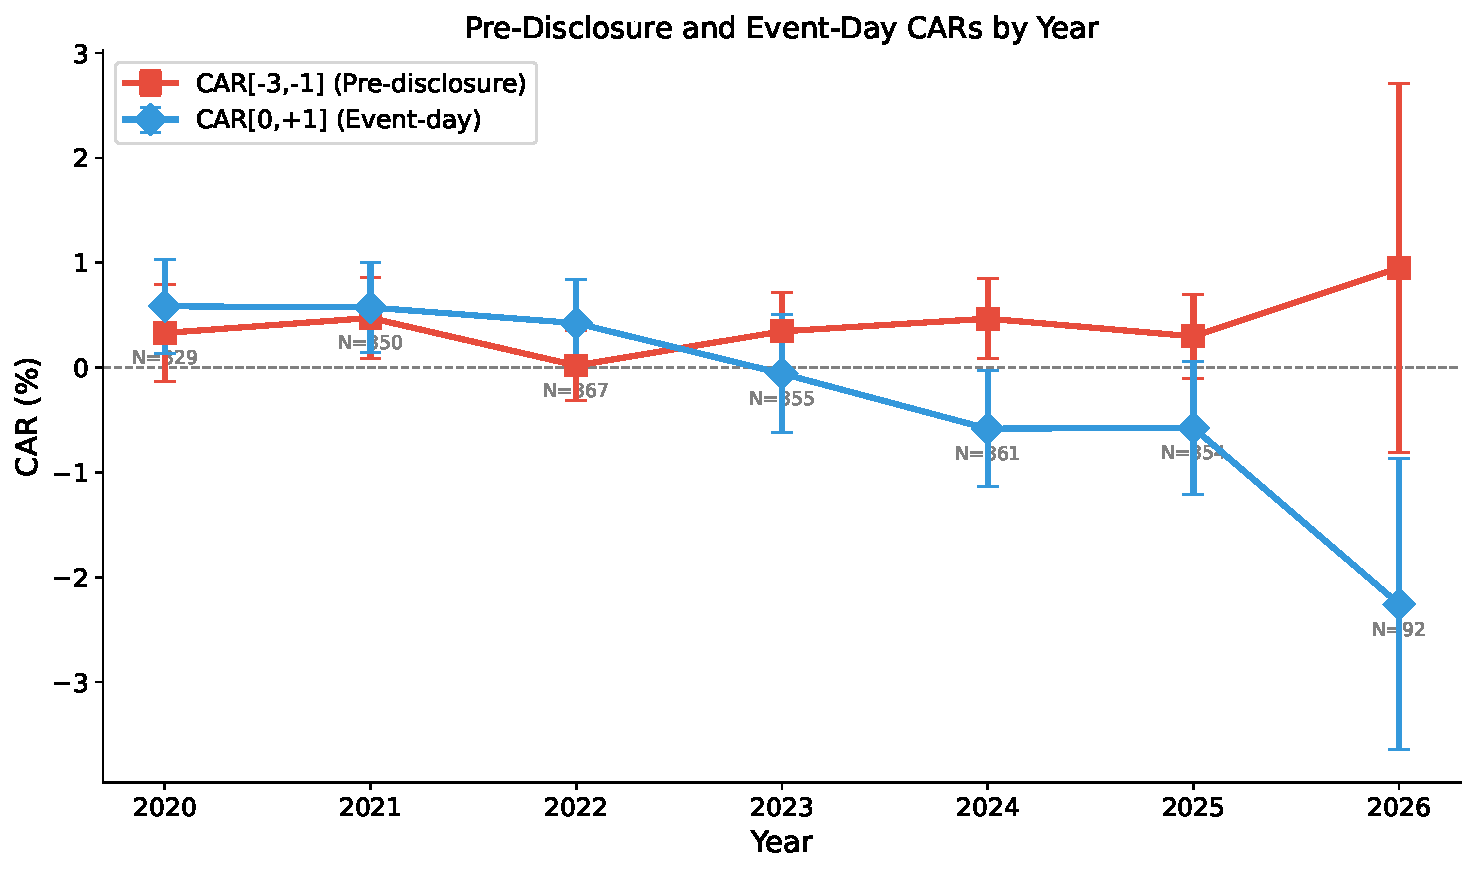
\includegraphics[width=0.85\textwidth]{figures/fig3_year.pdf}
\caption{Pre-disclosure CAR[-3,$-$1] and event-day CAR[0,+1] by year. The temporal shift reflects macroeconomic conditions rather than changes in information leakage.}
\label{fig:year}
\end{figure}

\subsection{Cross-sectional analysis by chaebol group}

The Korean market's chaebol structure provides a natural cross-sectional dimension for examining whether pre-disclosure drift varies systematically across corporate groups. If information leakage were concentrated in specific chaebols---perhaps due to weaker internal controls or more extensive analyst networks---we would expect significantly higher directional drift in those groups.

Table~\ref{tab:chaebol} reports CAR[-3,$-$1] and CAR[0,+1] by chaebol group. Pre-disclosure CARs range from $-$0.228\% (Doosan) to +1.565\% (Hanwha), with Hanwha's drift significantly higher than the rest ($t$=3.41, $p$<0.001). An ANOVA test across all 12 groups yields $F$=1.73 ($p$=0.062), suggesting marginally significant heterogeneity.

\begin{table}[ht]
\caption{Cumulative abnormal returns by chaebol group}
\label{tab:chaebol}
\begin{tabular}{lrrrrr}
\toprule
& & \multicolumn{2}{c}{CAR[-3,$-$1]} & \multicolumn{2}{c}{CAR[0,+1]} \\
\cmidrule(lr){3-4} \cmidrule(lr){5-6}
Chaebol & $N$ & Mean (\%) & $t$ & Mean (\%) & $t$ \\
\midrule
Hanwha & 116 & +1.565 & 2.30 & $-$0.583 & $-$0.81 \\
CJ & 75 & +0.881 & 1.98 & $-$0.120 & $-$0.16 \\
GS & 53 & +0.604 & 1.37 & +0.674 & 1.53 \\
Lotte & 92 & +0.517 & 1.33 & +0.202 & 0.36 \\
HD Hyundai & 497 & +0.474 & 2.38 & +0.312 & 1.42 \\
Samsung & 292 & +0.318 & 1.70 & +0.012 & 0.05 \\
LG & 185 & +0.278 & 1.22 & $-$0.311 & $-$0.81 \\
SK & 195 & +0.127 & 0.54 & $-$0.286 & $-$0.84 \\
Hyundai Motor & 402 & +0.093 & 0.52 & $-$0.352 & $-$1.62 \\
POSCO & 156 & +0.060 & 0.15 & $-$0.427 & $-$0.86 \\
KT & 80 & $-$0.006 & $-$0.03 & +1.310 & 4.25 \\
Doosan & 65 & $-$0.228 & $-$0.46 & $-$0.677 & $-$0.96 \\
\midrule
All & 2,208 & +0.347 & 4.04 & $-$0.042 & $-$0.39 \\
\bottomrule
\end{tabular}
\begin{flushleft}
\small Note: Sorted by descending CAR[-3,$-$1]. ANOVA across groups: $F$=1.73 ($p$=0.062) for CAR[-3,$-$1], $F$=1.29 ($p$=0.223) for CAR[0,+1].
\end{flushleft}
\end{table}

Fig.~\ref{fig:chaebol} visualizes the cross-sectional pattern. Hanwha's elevated drift likely reflects the defense sector's sensitivity to geopolitical news rather than information leakage about earnings specifically. KT exhibits remarkably high event-window returns (+1.310\%, $t$=4.25, $p$=0.027 vs.\ non-KT), consistent with telecommunications sector earnings surprises being particularly impactful. Samsung---despite being the most closely watched chaebol---shows only moderate pre-disclosure drift (+0.318\%).

\begin{figure}[ht]
\centering
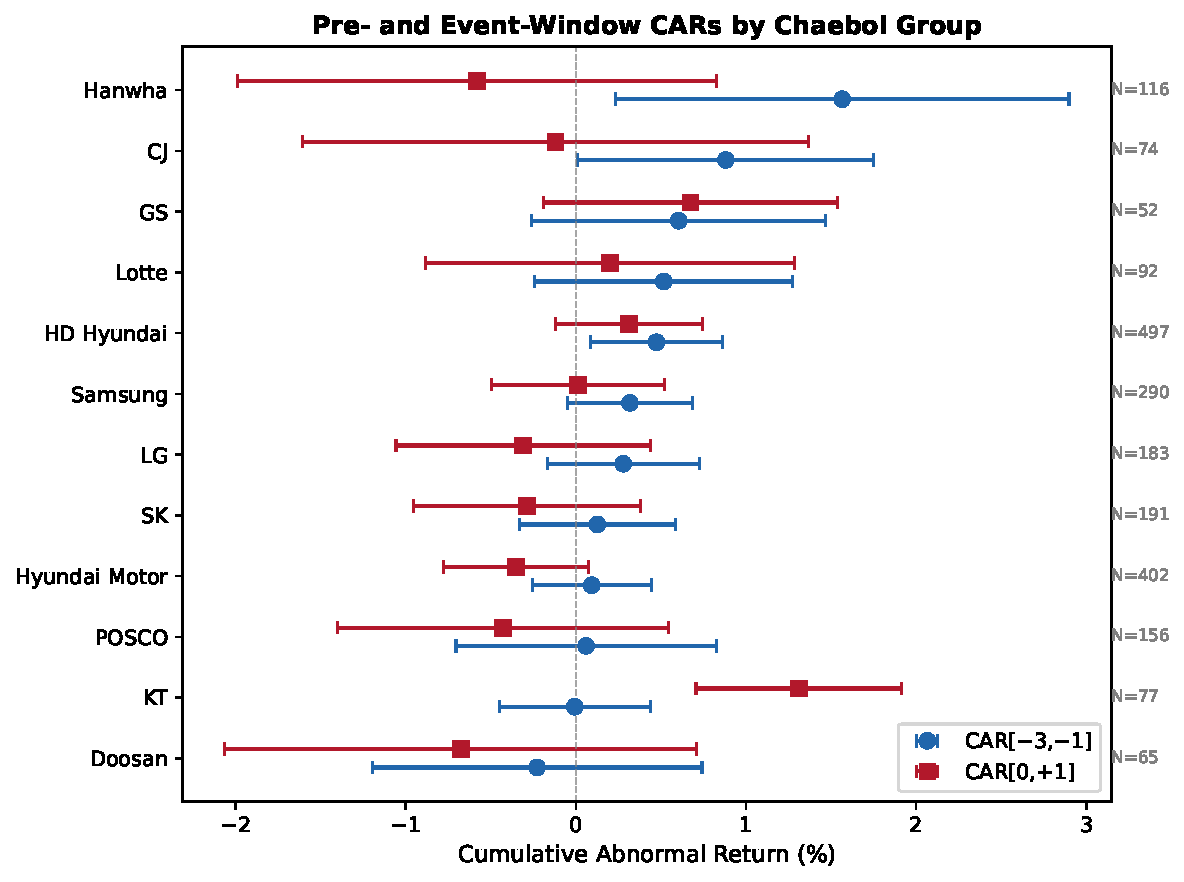
\includegraphics[width=0.95\textwidth]{figures/fig6_chaebol_car.pdf}
\caption{Pre-disclosure CAR[-3,$-$1] and event-window CAR[0,+1] by chaebol group with 95\% confidence intervals. Substantial cross-group variation exists, but no group shows patterns consistent with systematic directional information leakage.}
\label{fig:chaebol}
\end{figure}

Importantly, the cross-group variation does not exhibit the pattern expected under systematic information leakage. Pre-disclosure and event-window CARs are uncorrelated across groups (Spearman $\rho$=$-$0.14, $p$=0.668), suggesting that the drivers of pre-disclosure drift are distinct from the earnings information revealed at disclosure.

\subsection{Firm size and beta effects}

To investigate whether pre-disclosure drift varies with firm characteristics, we divide the sample into terciles by firm size (log market capitalization) and market beta. Table~\ref{tab:size_beta} reports CARs for each tercile.

\begin{table}[ht]
\caption{CARs by firm size and market beta terciles}
\label{tab:size_beta}
\begin{tabular}{lrrrrrr}
\toprule
& & \multicolumn{2}{c}{CAR[-3,$-$1]} & \multicolumn{2}{c}{CAR[0,+1]} & {CAR[-5,$-$1]} \\
\cmidrule(lr){3-4} \cmidrule(lr){5-6} \cmidrule(lr){7-7}
Tercile & $N$ & Mean (\%) & $t$ & Mean (\%) & $t$ & Mean (\%) \\
\midrule
\multicolumn{7}{l}{\textit{Panel A: Firm size terciles}} \\
Small & 790 & +0.403 & 2.91 & $-$0.058 & $-$0.32 & +0.578 \\
Medium & 726 & +0.374 & 2.45 & $-$0.005 & $-$0.03 & +0.590 \\
Large & 679 & +0.250 & 1.58 & $-$0.109 & $-$0.60 & +0.359 \\
\midrule
\multicolumn{7}{l}{\textit{Panel B: Market beta terciles}} \\
Low $\beta$ & 727 & +0.515 & 3.53 & $-$0.063 & $-$0.35 & +0.607 \\
Mid $\beta$ & 732 & +0.303 & 2.04 & $-$0.033 & $-$0.17 & +0.446 \\
High $\beta$ & 736 & +0.222 & 1.45 & $-$0.073 & $-$0.38 & +0.492 \\
\bottomrule
\end{tabular}
\begin{flushleft}
\small Note: Size tercile boundaries: Small (log size $\leq$ 12.56), Medium (12.56--13.45), Large ($>$ 13.64). Beta tercile boundaries: Low ($\beta \leq$ 0.845), Mid (0.845--1.129), High ($\beta >$ 1.130).
\end{flushleft}
\end{table}

Panel A reveals a monotonically decreasing relationship between firm size and pre-disclosure drift. However, the small-large difference is not statistically significant ($t$=0.92, $p$=0.358), and a Kruskal-Wallis test is also insignificant ($H$=2.88, $p$=0.237). Panel B shows a similar pattern for market beta. The Spearman correlation between beta and CAR[-3,$-$1] is $-$0.057 ($p$=0.008), indicating a statistically significant but economically modest negative relationship. Low-beta stocks may exhibit higher pre-disclosure drift because their lower systematic risk makes firm-specific information relatively more important.

\begin{figure}[ht]
\centering
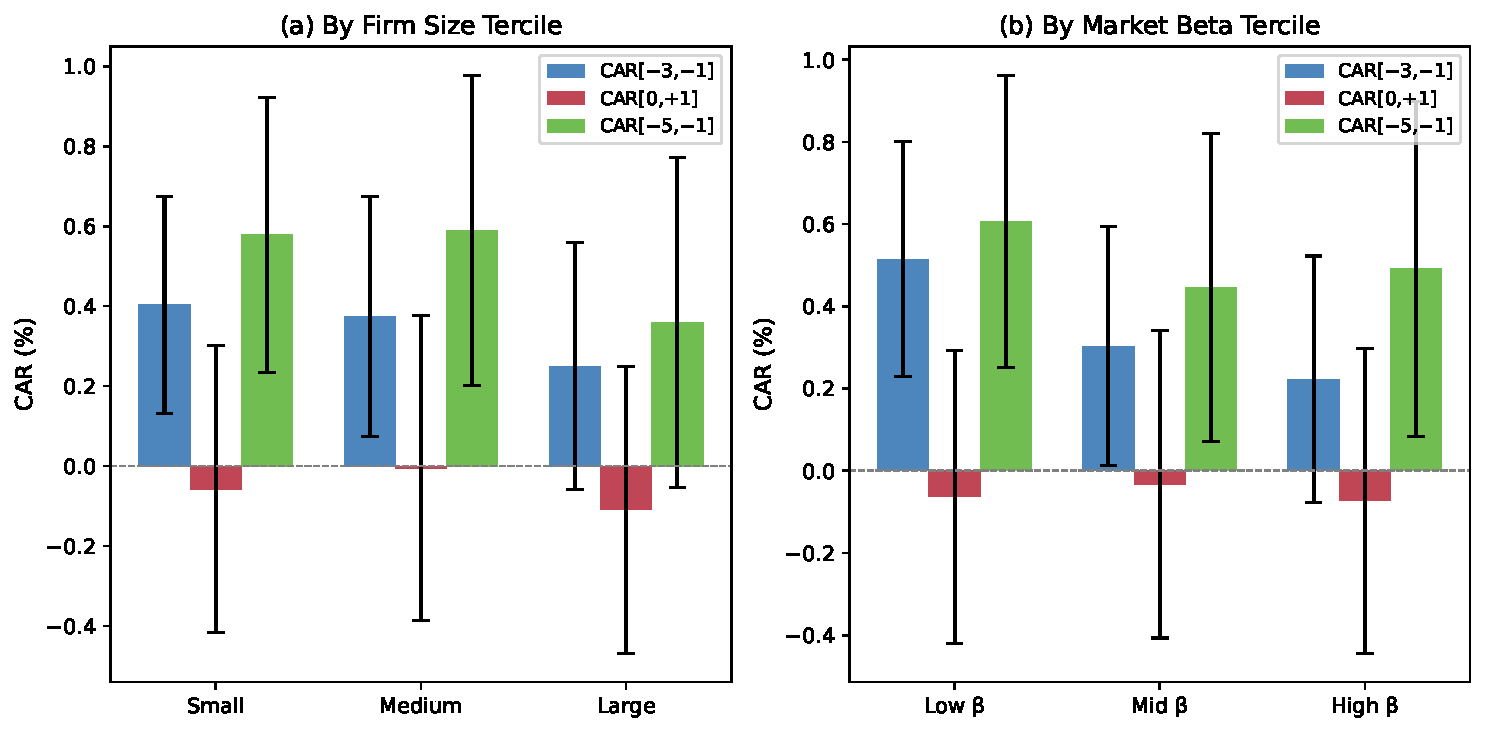
\includegraphics[width=0.95\textwidth]{figures/fig7_size_beta.pdf}
\caption{CARs by firm size tercile (Panel a) and market beta tercile (Panel b) with 95\% confidence intervals. Pre-disclosure drift is slightly larger for smaller and lower-beta firms, but event-window CARs are uniformly near zero across all terciles.}
\label{fig:size_beta}
\end{figure}

Event-window CARs (CAR[0,+1]) are uniformly close to zero across all size and beta terciles, confirming that the non-directional character of post-disclosure returns is not an artifact of pooling heterogeneous subsamples. These results are consistent with the well-documented size effect in pre-announcement drift \citep{atiase1985predisclosure}: smaller firms have less pre-disclosure information production, creating larger price adjustments when new information arrives.

\section{Discussion}
\label{sec:discussion}

\subsection{Drift without directional leakage}

Three complementary tests suggest the drift is non-directional: (1) direction test: 49.0\% accuracy; (2) non-parametric tests: sign test ($p$=0.585) and Wilcoxon ($p$=0.142) fail; (3) surprise conditioning: $p$=0.703. The drift appears driven by company-specific news unrelated to earnings, market momentum, or anticipatory trading based on publicly available signals. This interpretation is consistent with \citet{hirshleifer2003limited}, who argue that limited investor attention can produce predictable patterns without implying illegal information access.

The cross-sectional analyses reinforce this conclusion. While pre-disclosure drift varies across chaebol groups (Hanwha showing the highest at +1.565\%), this variation is uncorrelated with event-window returns, inconsistent with directional information leakage. The size and beta patterns---smaller and lower-beta firms showing modestly larger drift---reflect normal variation in information environments rather than differential insider access. The most parsimonious explanation combines positive market momentum during the sample period, right-skewed return distributions \citep{flannery2004partial}, and anticipatory non-directional trading \citep{chae2005trading}.

\subsection{Comparison with international evidence}

Our findings align with the broader evidence on fair disclosure regulation. \citet{bailey2003regulation} find that Reg FD reduced selective disclosure, and \citet{eleswarapu2004impact} document reduced information asymmetry. \citet{christensen2013capital} show that capital-market effects of securities regulation depend on prior institutional conditions and enforcement intensity. Our contribution is distinct: rather than evaluating the \textit{introduction} of fair disclosure, we test whether the regulation continues to be effective \textit{within} the regulated regime by examining directional content over a six-year window.

The Korean result contrasts with evidence from markets with weaker enforcement. \citet{beny2005impact} demonstrates that countries with stronger insider trading enforcement exhibit more efficient stock prices, and \citet{leuz2003earnings} find that investor protection is associated with lower earnings management. Korea's combination of mandatory electronic filing, strict enforcement by the Financial Supervisory Service, and concentrated analyst coverage appears to create an institutional environment where directional information leakage is effectively deterred.

\subsection{Methodological contributions}

This study makes several methodological contributions. First, we demonstrate the importance of \textbf{multi-test triangulation} in event studies. The parametric $t$-test implicitly assumes normally distributed abnormal returns. When the distribution is right-skewed, the parametric mean is inflated by outliers, producing significant $t$-statistics even when the majority of events show no drift. The sign test and Wilcoxon signed-rank test provide a more accurate characterization of the typical event.

Second, we introduce the \textbf{directional conditioning test} as a direct diagnostic for information leakage. Prior event studies typically interpret significant pre-announcement drift as evidence of informed trading without verifying whether the drift predicts the direction of the subsequent news. This test could be adopted as a standard diagnostic in future event studies.

Third, we document the importance of \textbf{filing time classification}. The finding that 96.5\% of DART filings occur after market close implies that Day~0 returns are effectively pre-disclosure. Studies that attribute Day~0 returns to information release may be misinterpreting anticipatory trading as immediate market reaction.

\subsection{Implications for policy and practice}

For regulators, non-directional drift suggests Korea's Fair Disclosure regime does not require fundamental reform. Material earnings information reaches the market simultaneously, and prices respond correctly only upon public disclosure. For investors, post-disclosure Day~+1 returns correctly price surprises with 60.6\% accuracy ($p$<0.001), while pre-disclosure drift strategies are unlikely to be profitable directionally.

\subsection{Limitations}

Several limitations warrant discussion. First, our YoY operating profit change as a surprise measure is crude compared to the analyst consensus forecast standard \citep{livnat2006comparing}. Only 26.4\% of events yield parseable surprises, and parseable events come from larger firms with lower beta. Second, our sample is limited to 64 large chaebol affiliates; information leakage may be more prevalent among smaller, less scrutinized firms. Third, Korean Fama-French factors are unavailable, preventing multi-factor benchmark models. Fourth, we cannot rule out that pre-disclosure volume increases reflect legal mosaic information assembly. Fifth, our analysis focuses on earnings disclosures and does not examine other material events where leakage incentives may differ.

\section{Conclusion}
\label{sec:conclusion}

This study finds no evidence of directional information leakage in Korean earnings announcements. Three independent analyses converge: direction prediction accuracy of 49.0\% (no better than chance), failure of non-parametric tests to confirm parametric drift (sign test $p$=0.585; Wilcoxon $p$=0.142), and surprise-conditioned CARs that are indistinguishable by earnings direction ($p$=0.703). The first post-disclosure trading day shows a strong, correct directional response (60.6\% accuracy, $p$<0.001), confirming that material earnings information is incorporated into prices only upon public release through the DART system.

Cross-sectional analyses reveal significant heterogeneity across chaebol groups, firm sizes, and market betas, but these patterns are consistent with normal variation in information environments rather than differential information leakage. The most-watched chaebol group (Samsung) shows only moderate, non-directional drift.

Our results carry a broader methodological lesson: pre-announcement drift should not be conflated with information leakage without conditioning on the direction of the actual news \citep{meulbroek1992comparison, bernile2016can, atiase1985predisclosure}. Future work should extend the analysis to non-chaebol firms and incorporate analyst consensus surprises.

\section*{Acknowledgments}

The author thanks the DART electronic disclosure system for providing publicly accessible corporate filing data. All disclosure data are publicly available through DART (\url{https://dart.fss.or.kr}). Stock price data are from KRX via FinanceDataReader. Analysis code is available at \url{[Available upon publication]}.

\bibliographystyle{elsarticle-harv}
\bibliography{refs}

\end{document}
